\documentclass[border=6pt]{standalone}
\usepackage{amsmath}
\usepackage{tikz}
\usetikzlibrary{arrows.meta}
\begin{document}
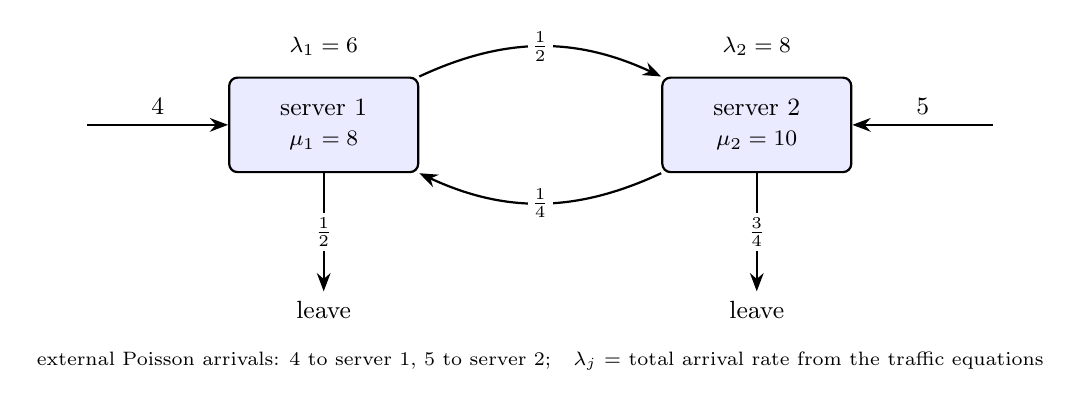
\begin{tikzpicture}[>=Stealth,font=\small,
 s/.style={draw,thick,circle,minimum size=1.1cm,inner sep=0pt,fill=blue!8},
 e/.style={->,thick},
 lab/.style={font=\small,fill=white,inner sep=1.5pt},
 every loop/.style={->,thick,looseness=6}]
\tikzset{st/.style={draw,thick,rounded corners=3pt,fill=blue!8,align=center,minimum width=2.4cm,minimum height=1.2cm}}
\node[st] (1) at (0,0) {server 1\\{\footnotesize $\mu_1=8$}};
\node[st] (2) at (5.5,0) {server 2\\{\footnotesize $\mu_2=10$}};
\draw[e] (-3,0) -- node[above]{4} (1);
\draw[e] (8.5,0) -- node[above]{5} (2);
\draw[e] (1.north east) to[bend left=25] node[lab]{$\tfrac12$} (2.north west);
\draw[e] (2.south west) to[bend left=25] node[lab]{$\tfrac14$} (1.south east);
\draw[e] (1.south) -- node[lab]{$\tfrac12$} ++(0,-1.5) node[below]{leave};
\draw[e] (2.south) -- node[lab]{$\tfrac34$} ++(0,-1.5) node[below]{leave};
\node[font=\footnotesize] at (0,1.0) {$\lambda_1=6$};
\node[font=\footnotesize] at (5.5,1.0) {$\lambda_2=8$};
\node[font=\scriptsize,align=center] at (2.75,-3.0) {external Poisson arrivals: 4 to server 1, 5 to server 2;\quad $\lambda_j$ = total arrival rate from the traffic equations};
\end{tikzpicture}
\end{document}
